\documentclass[aspectratio=169]{beamer}
\usetheme{Madrid}
\setbeamertemplate{navigation symbols}{}

\usepackage{booktabs}
\usepackage{graphicx}

\title{Cameroon Main Results}
\subtitle{Cleaning diagnostics and NACAM employment elasticities}
\author{}
\date{\today}

\begin{document}

\begin{frame}
    \titlepage
\end{frame}

\begin{frame}{Roadmap}
    \tableofcontents
\end{frame}

\section{BDF Cleaning Results}

\begin{frame}{Why Cleaning Choices Matter}
    \begin{itemize}
        \item The working panel is organized at the firm-year level, so duplicate handling changes both sample size and identification.
        \item Sector harmonization matters because the elasticity analysis is estimated separately across observed NACAM branches.
        \item The cleaning note isolates the two steps that most affect downstream interpretation: duplicate resolution and the NACAM-to-ISIC crosswalk.
    \end{itemize}
\end{frame}

\begin{frame}{Firm-Year Duplicate Cleaning}
    \footnotesize
    \begin{itemize}
        \item Working key: \texttt{firmid} $\times$ \texttt{fin\_yr}
        \item Perfect duplicates would be collapsed with original row order as the tie-breaker.
        \item Conflicting duplicate firm-years are fully removed from the cleaned analysis file.
    \end{itemize}

    \vspace{0.2cm}
    \centering
    \resizebox{0.76\textwidth}{!}{
        \begin{tabular}{lr}
                        &       Value\\
\midrule
Original observations&       9,325\\
Perfect duplicate firm-years&           0\\
Rows dropped from perfect duplicates&           0\\
Conflicting duplicate firm-years&         127\\
Rows dropped from conflicting duplicates&         257\\
Final cleaned observations&       9,068\\

        \end{tabular}
    }
\end{frame}

\begin{frame}{NACAM-to-ISIC Crosswalk}
    \small
    \begin{itemize}
        \item Observed legacy NACAM codes are audited directly from the Cameroon BDF file.
        \item ISIC Rev.4 divisions are assigned only when the official mapping is one-to-one.
        \item Ambiguous branches remain flagged for manual review rather than being forced into a noisy division code.
    \end{itemize}

    \vspace{0.4cm}
    \centering
    \resizebox{0.75\textwidth}{!}{
        \begin{tabular}{lr}
                        &       Value\\
\midrule
Observed legacy NACAM codes covered&          37\\
Codes with exact ISIC Rev.4 division assignment&          17\\
Codes flagged for manual review&          20\\

        \end{tabular}
    }
\end{frame}

\begin{frame}{Cleaning Takeaways}
    \begin{itemize}
        \item The cleaned panel falls from 9,325 to 9,068 observations after removing conflicting duplicate firm-years.
        \item There are 127 conflicting firm-years, accounting for 257 dropped rows. Those observations are excluded rather than resolved ad hoc.
        \item The crosswalk covers 37 observed legacy NACAM codes, but only 17 map cleanly to a single ISIC Rev.4 division.
        \item The remaining 20 codes are explicitly flagged for manual review, which keeps sector harmonization transparent before pooled industry comparisons.
    \end{itemize}
\end{frame}

\section{NACAM Elasticity Results}

\begin{frame}{Specification and Sample}
    \small
    \begin{itemize}
        \item Unit of observation: firm-year in \texttt{Data/Analysis/CMR\_BDF\_cleaned.dta}
        \item Outcomes: log employment regressed on log value added and log total revenue in separate specifications.
        \item Sector heterogeneity: each model interacts the elasticity term with observed NACAM codes.
        \item Controls: firm fixed effects and NACAM-by-year effects.
        \item Inference: standard errors clustered at the firm level.
        \item Inclusion rule for reported sectors: at least 30 observations and 10 firms in both outcome samples.
    \end{itemize}
\end{frame}

\begin{frame}{Employment Distribution by Fiscal Year}
    \centering
    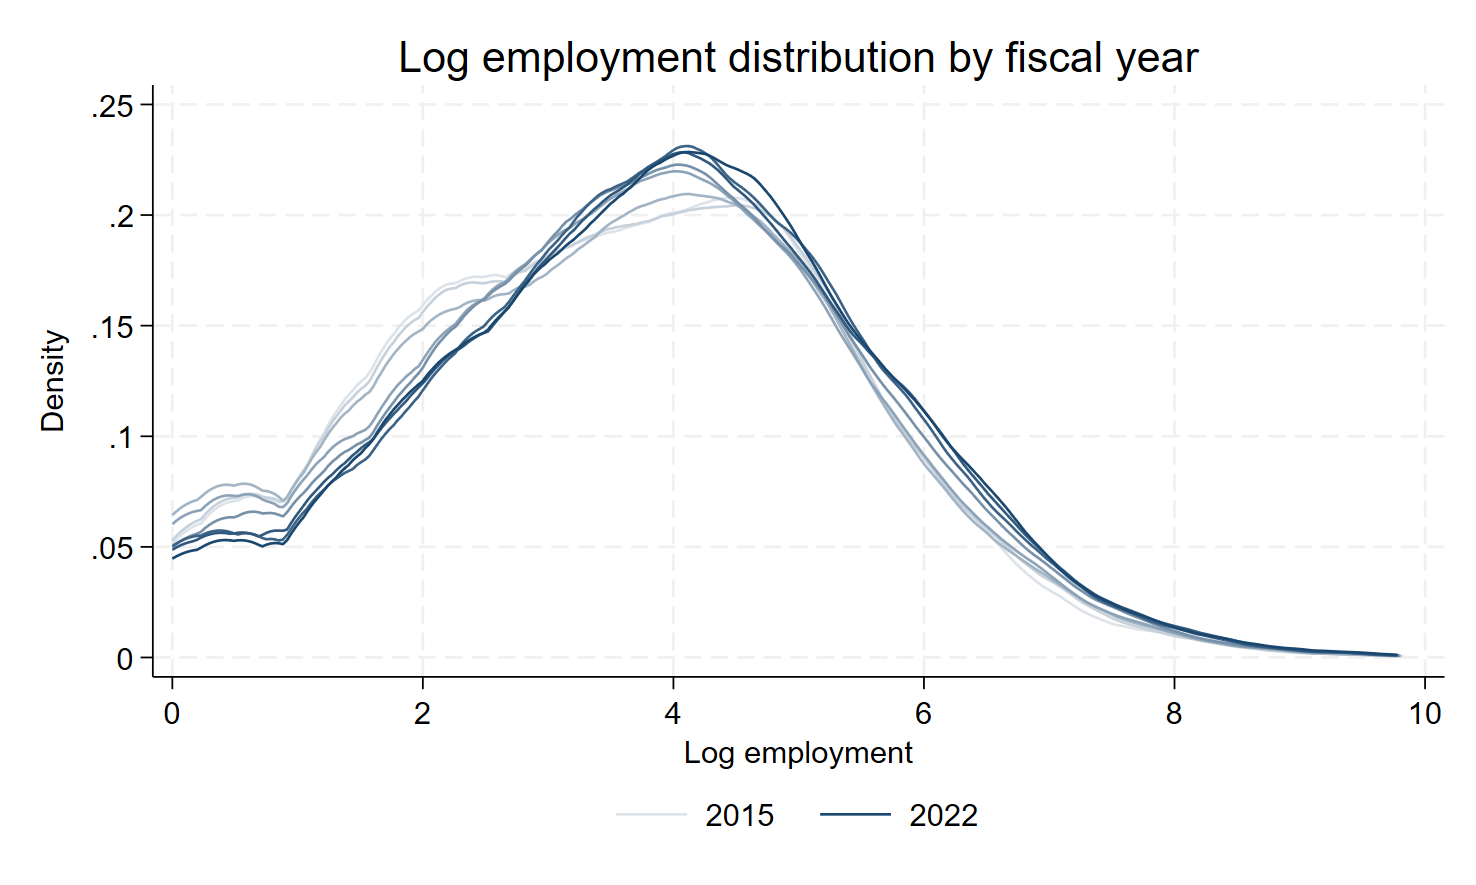
\includegraphics[width=\textwidth,height=0.76\textheight,keepaspectratio]{../output/figures/cmr_nacam_results_ln_emp_density_by_year.png}
\end{frame}

\begin{frame}{Main Elasticity Estimates Across NACAM Sectors}
    \centering
    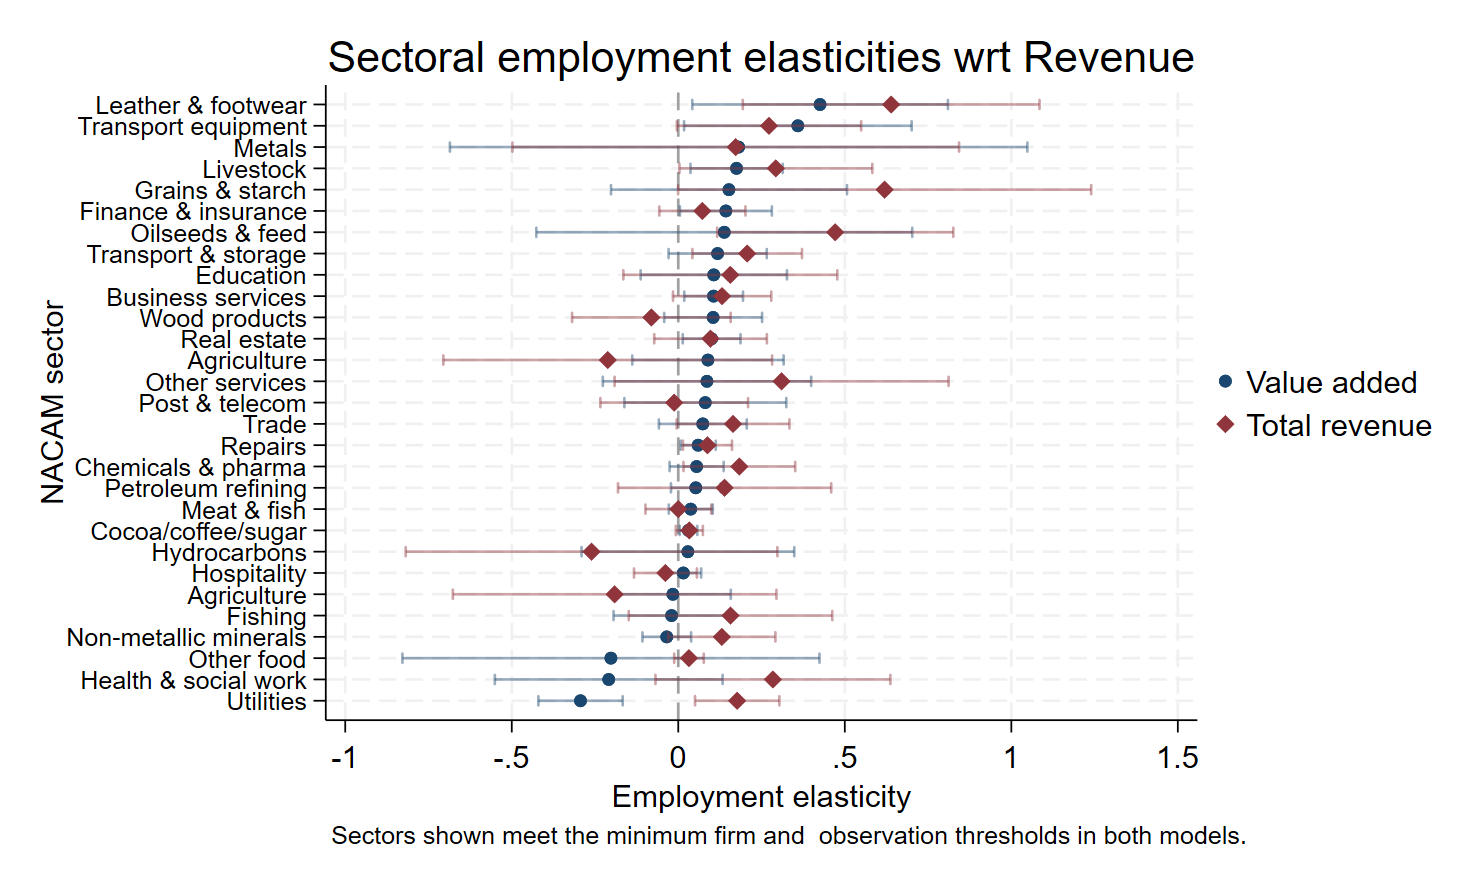
\includegraphics[width=\textwidth,height=0.76\textheight,keepaspectratio]{../output/figures/cmr_nacam_results_coefficients.png}
\end{frame}

\begin{frame}{Cross-Model Consistency}
    \centering
    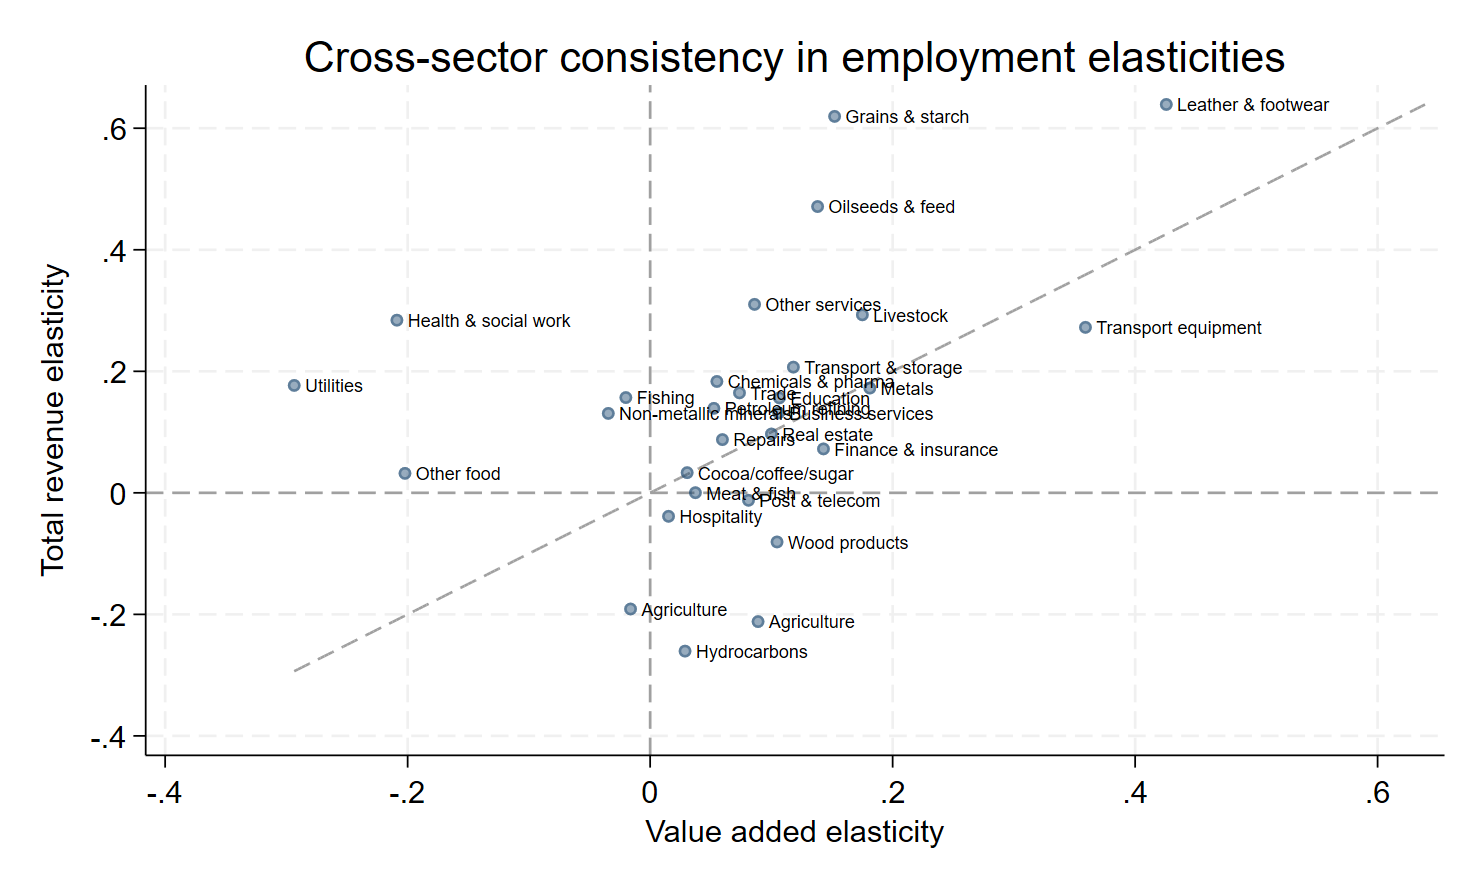
\includegraphics[width=\textwidth,height=0.76\textheight,keepaspectratio]{../output/figures/cmr_nacam_results_scatter.png}
\end{frame}

\begin{frame}{Selected Sectors From the VA Ranking}
    \small
    \begin{itemize}
        \item Table shows the top three and bottom two sectors by value-added elasticity.
        \item Total-revenue elasticities are included as a cross-check on whether the signal is consistent across revenue concepts.
    \end{itemize}

    \vspace{0.3cm}
    \centering
    \resizebox{\textwidth}{!}{
        \begin{tabular}{lrrrr}
            \input{../output/tables/cmr_nacam_results_highlights.tex}
        \end{tabular}
    }
\end{frame}

\begin{frame}{Main Takeaways}
    \begin{itemize}
        \item Elasticities vary meaningfully across NACAM sectors rather than lining up around a single Cameroon-wide coefficient.
        \item Several sectors show positive employment responses under both value added and total revenue, with NACAM 17 standing out most clearly.
        \item Negative or weak value-added elasticities remain concentrated in a small set of sectors, which is useful for prioritizing follow-up diagnostics.
        \item The cleaning and harmonization steps are not bookkeeping only; they determine which firm-years and sector codes enter the elasticity analysis.
    \end{itemize}
\end{frame}

\end{document}
